\documentclass{standalone}
\usepackage{tikz}
\begin{document}
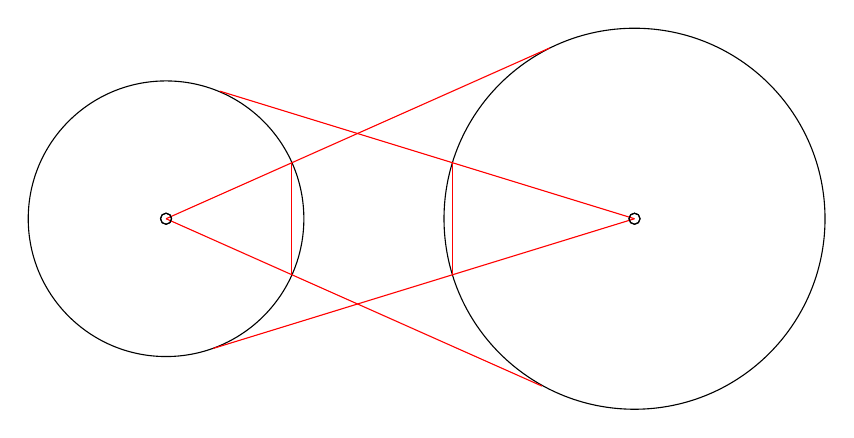
\begin{tikzpicture}[x=1pt,y=1pt]
\draw (225.90,-97.67) circle (68.84);
\draw (56.62,-97.67) circle (49.80);
\draw[red] (225.90,-97.67) -- (76.03,-51.55);
\draw[red] (225.90,-97.67) -- (73.68,-144.53);
\draw[red] (56.62,-97.67) -- (195.33,-35.93);
\draw[red] (56.62,-97.67) -- (192.46,-158.14);
\draw (225.90,-97.67) circle (2.00);
\draw (225.90,-97.67) circle (2.00);
\draw (56.62,-97.67) circle (2.00);
\draw (56.62,-97.67) circle (2.00);
\draw[red] (102.11,-77.42) -- (102.11,-117.92);
\draw[red] (160.11,-77.42) -- (160.11,-117.92);
\end{tikzpicture}
\end{document}
